\clearpage
\appendix
\section{Supplementary material}
\subsection{Prompt given to \astra}
System message:
\begin{lstlisting}
You are an engineering drafting and analysis assistant. Use your own reasoning; no external tools are provided. Do not claim you ran a solver.
\end{lstlisting}
User message for a circuit task, verbatim up to the source SVG, which follows in full:
\begin{lstlisting}
Instruction: Set R3 to 150 (*@$\Omega$@*).

Drawing conventions: straight lines are ideal wires. A wire that ends on another wire (a T) is connected to it; a filled dot also marks a connection; wires that cross without a dot are NOT connected. Rectangles are resistors and circles are ideal DC voltage sources; the '+' inside a source marks its positive terminal. Labels give component names and values.
Criteria (from the drawing notes): every resistor's dissipated power must not exceed the stated rating, and the magnitude of every source's current must not exceed the stated supply fuse rating.

Tasks:
1. Apply the instruction to the drawing, changing nothing else, and return the complete edited SVG.
2. Analyse the EDITED design and report whether it meets every criterion.

Answer with exactly two fenced blocks and nothing else: first ```svg containing the full edited SVG, then ```json containing {"verdict": "pass" or "fail", "violations": [names of every resistor or source that violates a criterion], "source_currents_A": {"V1": current delivered out of its + terminal, ...}, "max_resistor_power_W": {"name": "R?", "value": watts}}

Source SVG:
[complete source SVG]
\end{lstlisting}
For pipe networks the conventions paragraph and the JSON schema are replaced by:
\begin{lstlisting}
Drawing conventions: heavy lines are pipes; filled dots are junctions. A pipe runs between junctions or reservoirs and may turn through 90-degree elbows; each elbow adds the minor-loss coefficient K given in the notes. 'P# L m (*@\O{}@*)D' gives a pipe's length (m) and internal diameter (mm); 'J# q=.. L/s z=.. m' gives the demand withdrawn at a junction and its elevation; 'R# H=.. m' is a reservoir's fixed total head.
Analysis model: steady incompressible water, density 998 kg/m3, dynamic viscosity 1.002e-3 Pa s, g = 9.80665 m/s2; Darcy-Weisbach head loss with the Churchill (1977) friction factor and the pipe roughness in the notes; tee and junction losses neglected; pressure head at a junction = hydraulic head minus elevation.
Criteria (from the drawing notes): every pipe velocity must not exceed the maximum velocity, and every junction pressure head must be at least the minimum pressure head.

JSON schema: {"verdict": "pass" or "fail", "violations": [names of every pipe or junction that violates a criterion], "pipe_velocities_m_s": {"P1": speed, ...}, "min_pressure_head_m": {"name": "J?", "value": metres}}
\end{lstlisting}

\subsection{Worked \astra failure on the returned drawing}
\Cref{fig:astra-worked} shows the actual source SVG and \astra's returned SVG for the one completed network
answer with a substantive wrong verdict. The edit changes only P9's length from 290 to 340\,m; the returned
drawing equals the target SVG exactly. The source is already below its 20\,m pressure minimum at J4
(19.26\,m), and re-solving the edited SVG gives 19.23\,m. \astra instead reports 20.04\,m and \code{pass}.
Its reported velocity for P4 is 0.031\,m/s versus 0.095\,m/s from the edited drawing. These are analysis
errors on a correctly edited artifact. The orange and red marks in the figure are presentation overlays
added after the SVG was scored; they are not input to the verifier.

\begin{figure*}[t]
\centering
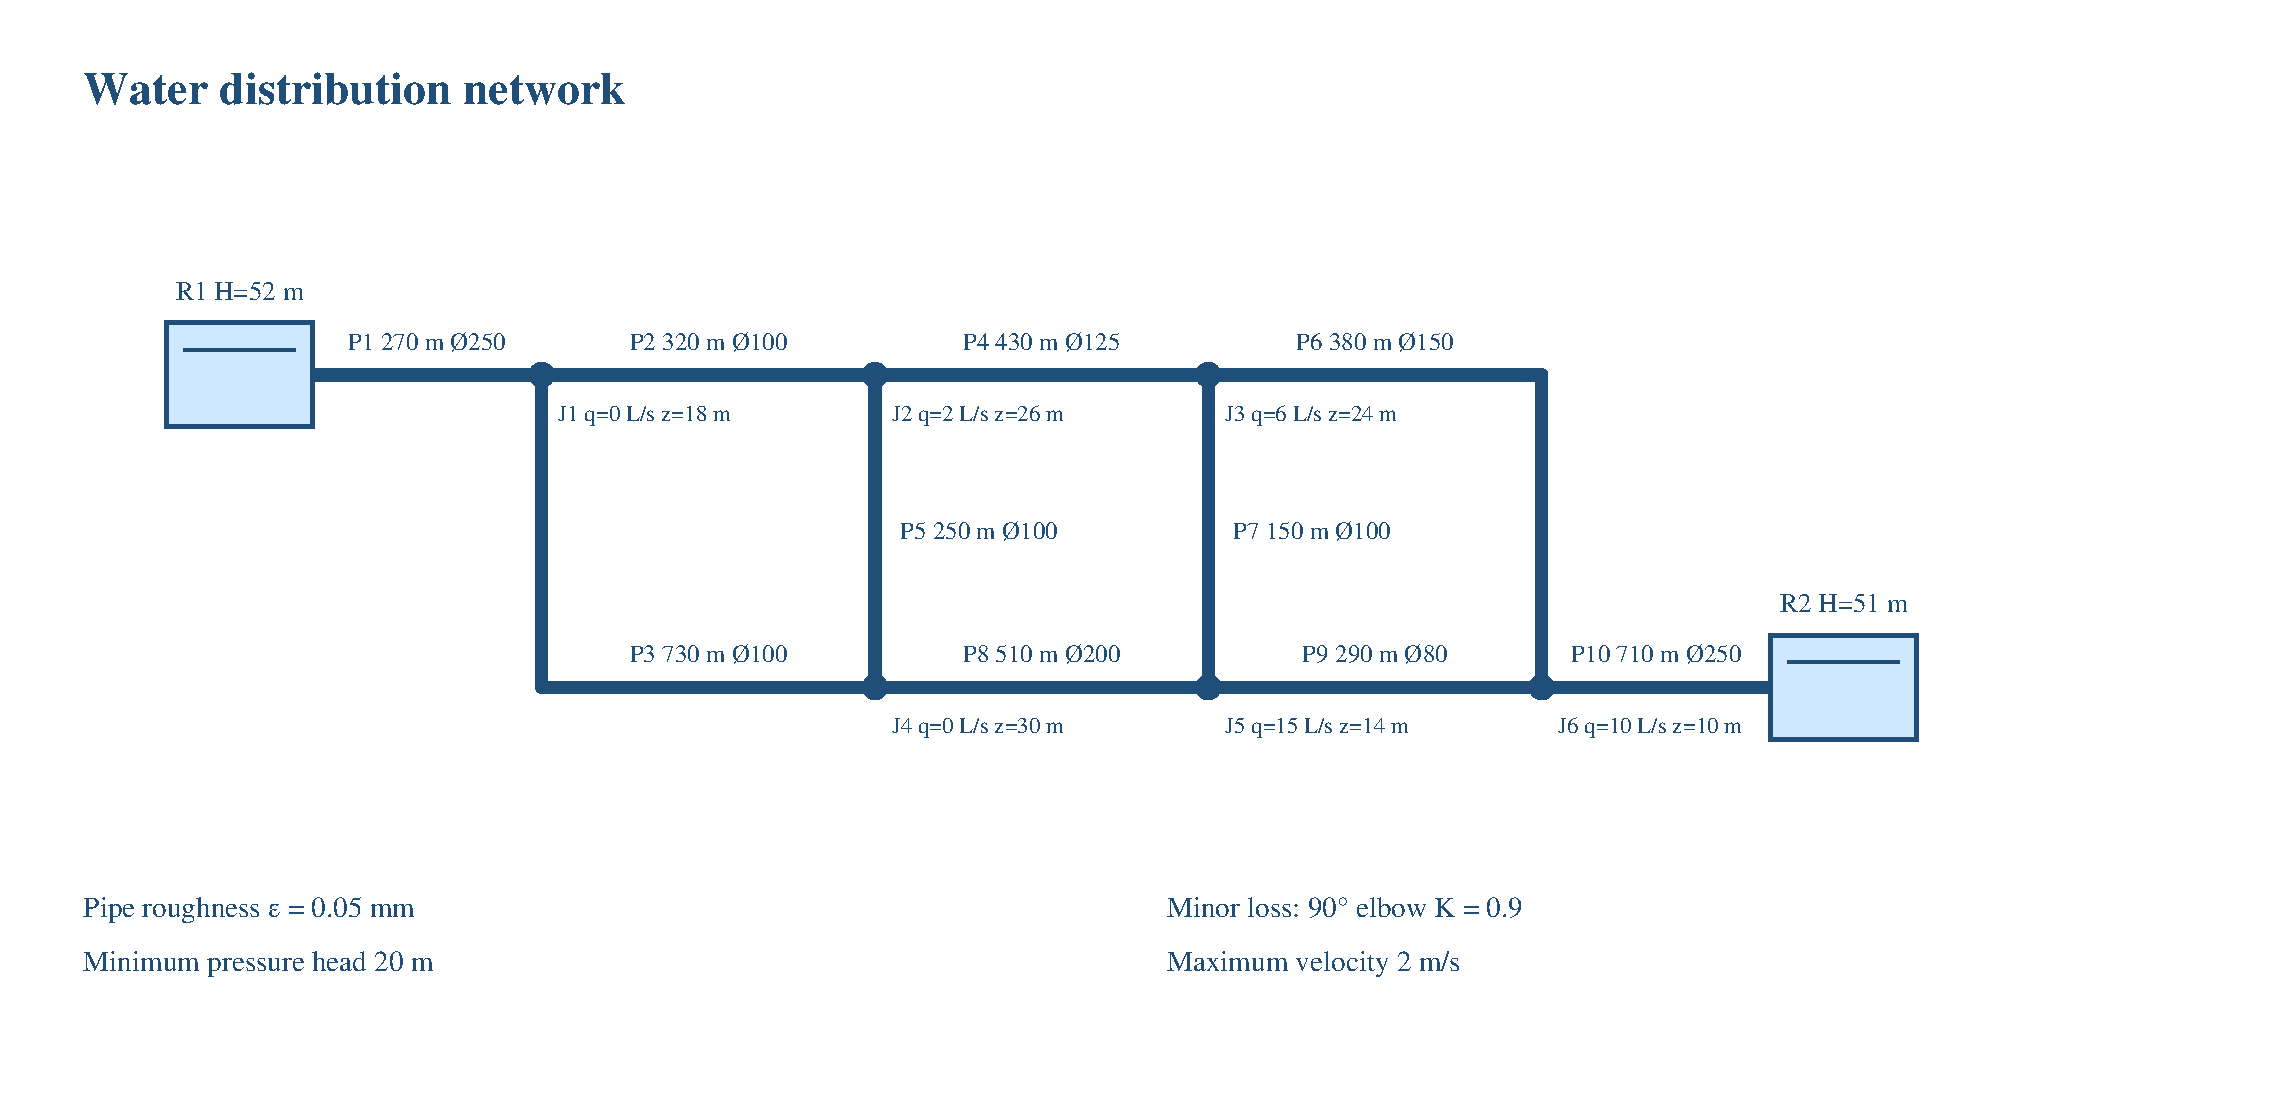
\includegraphics[width=.92\textwidth]{figures/astra-failure-source.pdf}\\[-2pt]
{\footnotesize (a) Source drawing: P9 is 290\,m; J4 is already below its pressure limit.}\\[3pt]
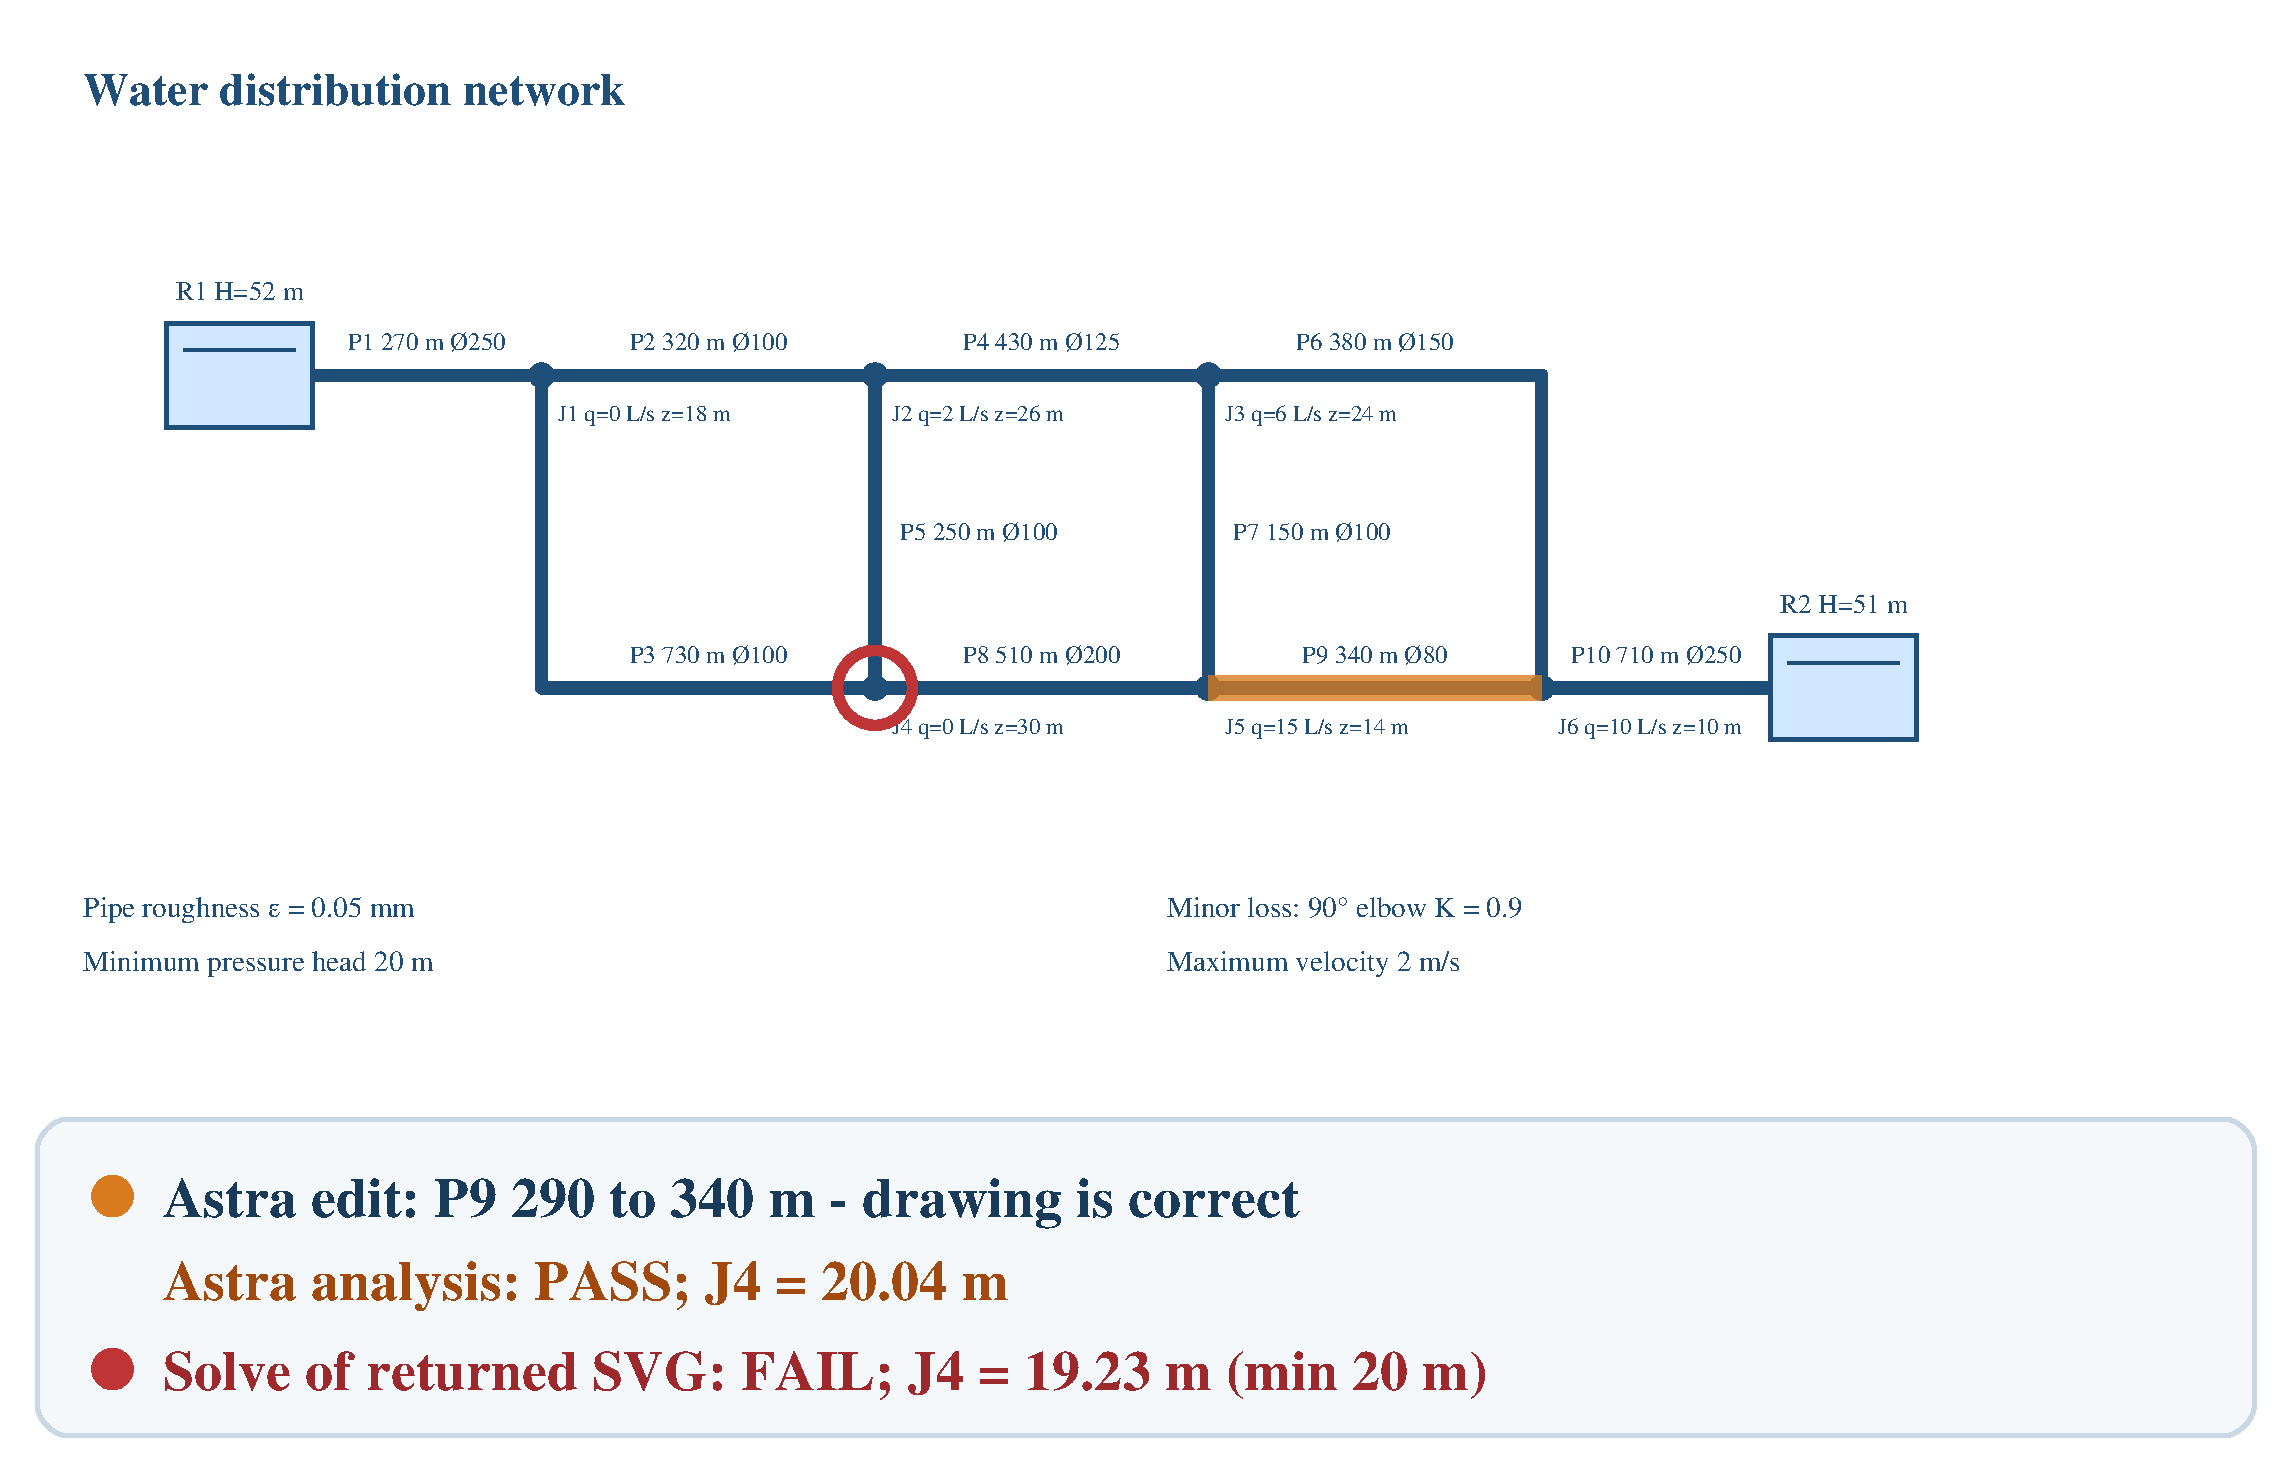
\includegraphics[width=.92\textwidth]{figures/astra-failure-response-annotated.pdf}\\[-2pt]
{\footnotesize (b) \astra's correct SVG edit (orange P9) with the missed J4 violation (red).}
\caption{\textbf{Astra failure, shown on the complete engineering drawings.} The two-reservoir, four-loop
network is edited correctly, but \astra's numerical answer declares it safe. The lower annotation contrasts
that answer with an independent solve of the returned SVG. Original unannotated SVGs were used for scoring.}
\label{fig:astra-worked}
\end{figure*}

\subsection{Separate structural-frame diagnostic}
To test whether the focus on circuits and pipe networks hid other engineering-drawing difficulties, we
re-audited saved \astra responses from a separate planar-frame study. The edit in
\cref{fig:astra-frame} moves one column grid from 3300 to 4000\,mm and increases the downward load at
the top-right joint from 53 to 68\,kN. The 21-member, three-storey frame has 27 degrees of static
indeterminacy. Its prompt supplied the explicit physical graph as well as the source SVG, and no
external solver. In three of four completed attempts on this same edit, \astra returned a drawing
whose member geometry and dimensions pass the independent scorer, but explicitly marked displacement
and stress as unavailable. In the fourth it gave values within 2\,\% of the frame FEM reference.
Re-solving each returned drawing gives $u_x=3.5119$\,mm, $u_y=-0.1882$\,mm and peak stress
$17.6837$\,MPa. This is a repeated refusal to calculate, not a wrong numerical safety claim.
It uses a separate planar-frame FEM harness; \ours does not verify these frames. Ten completed
mechanical CAD hard-screen tasks and six functional frame-sizing controls also passed their
respective saved-output audits, so neither provides an additional confirmed shape failure.

\begin{figure*}[t]
\centering
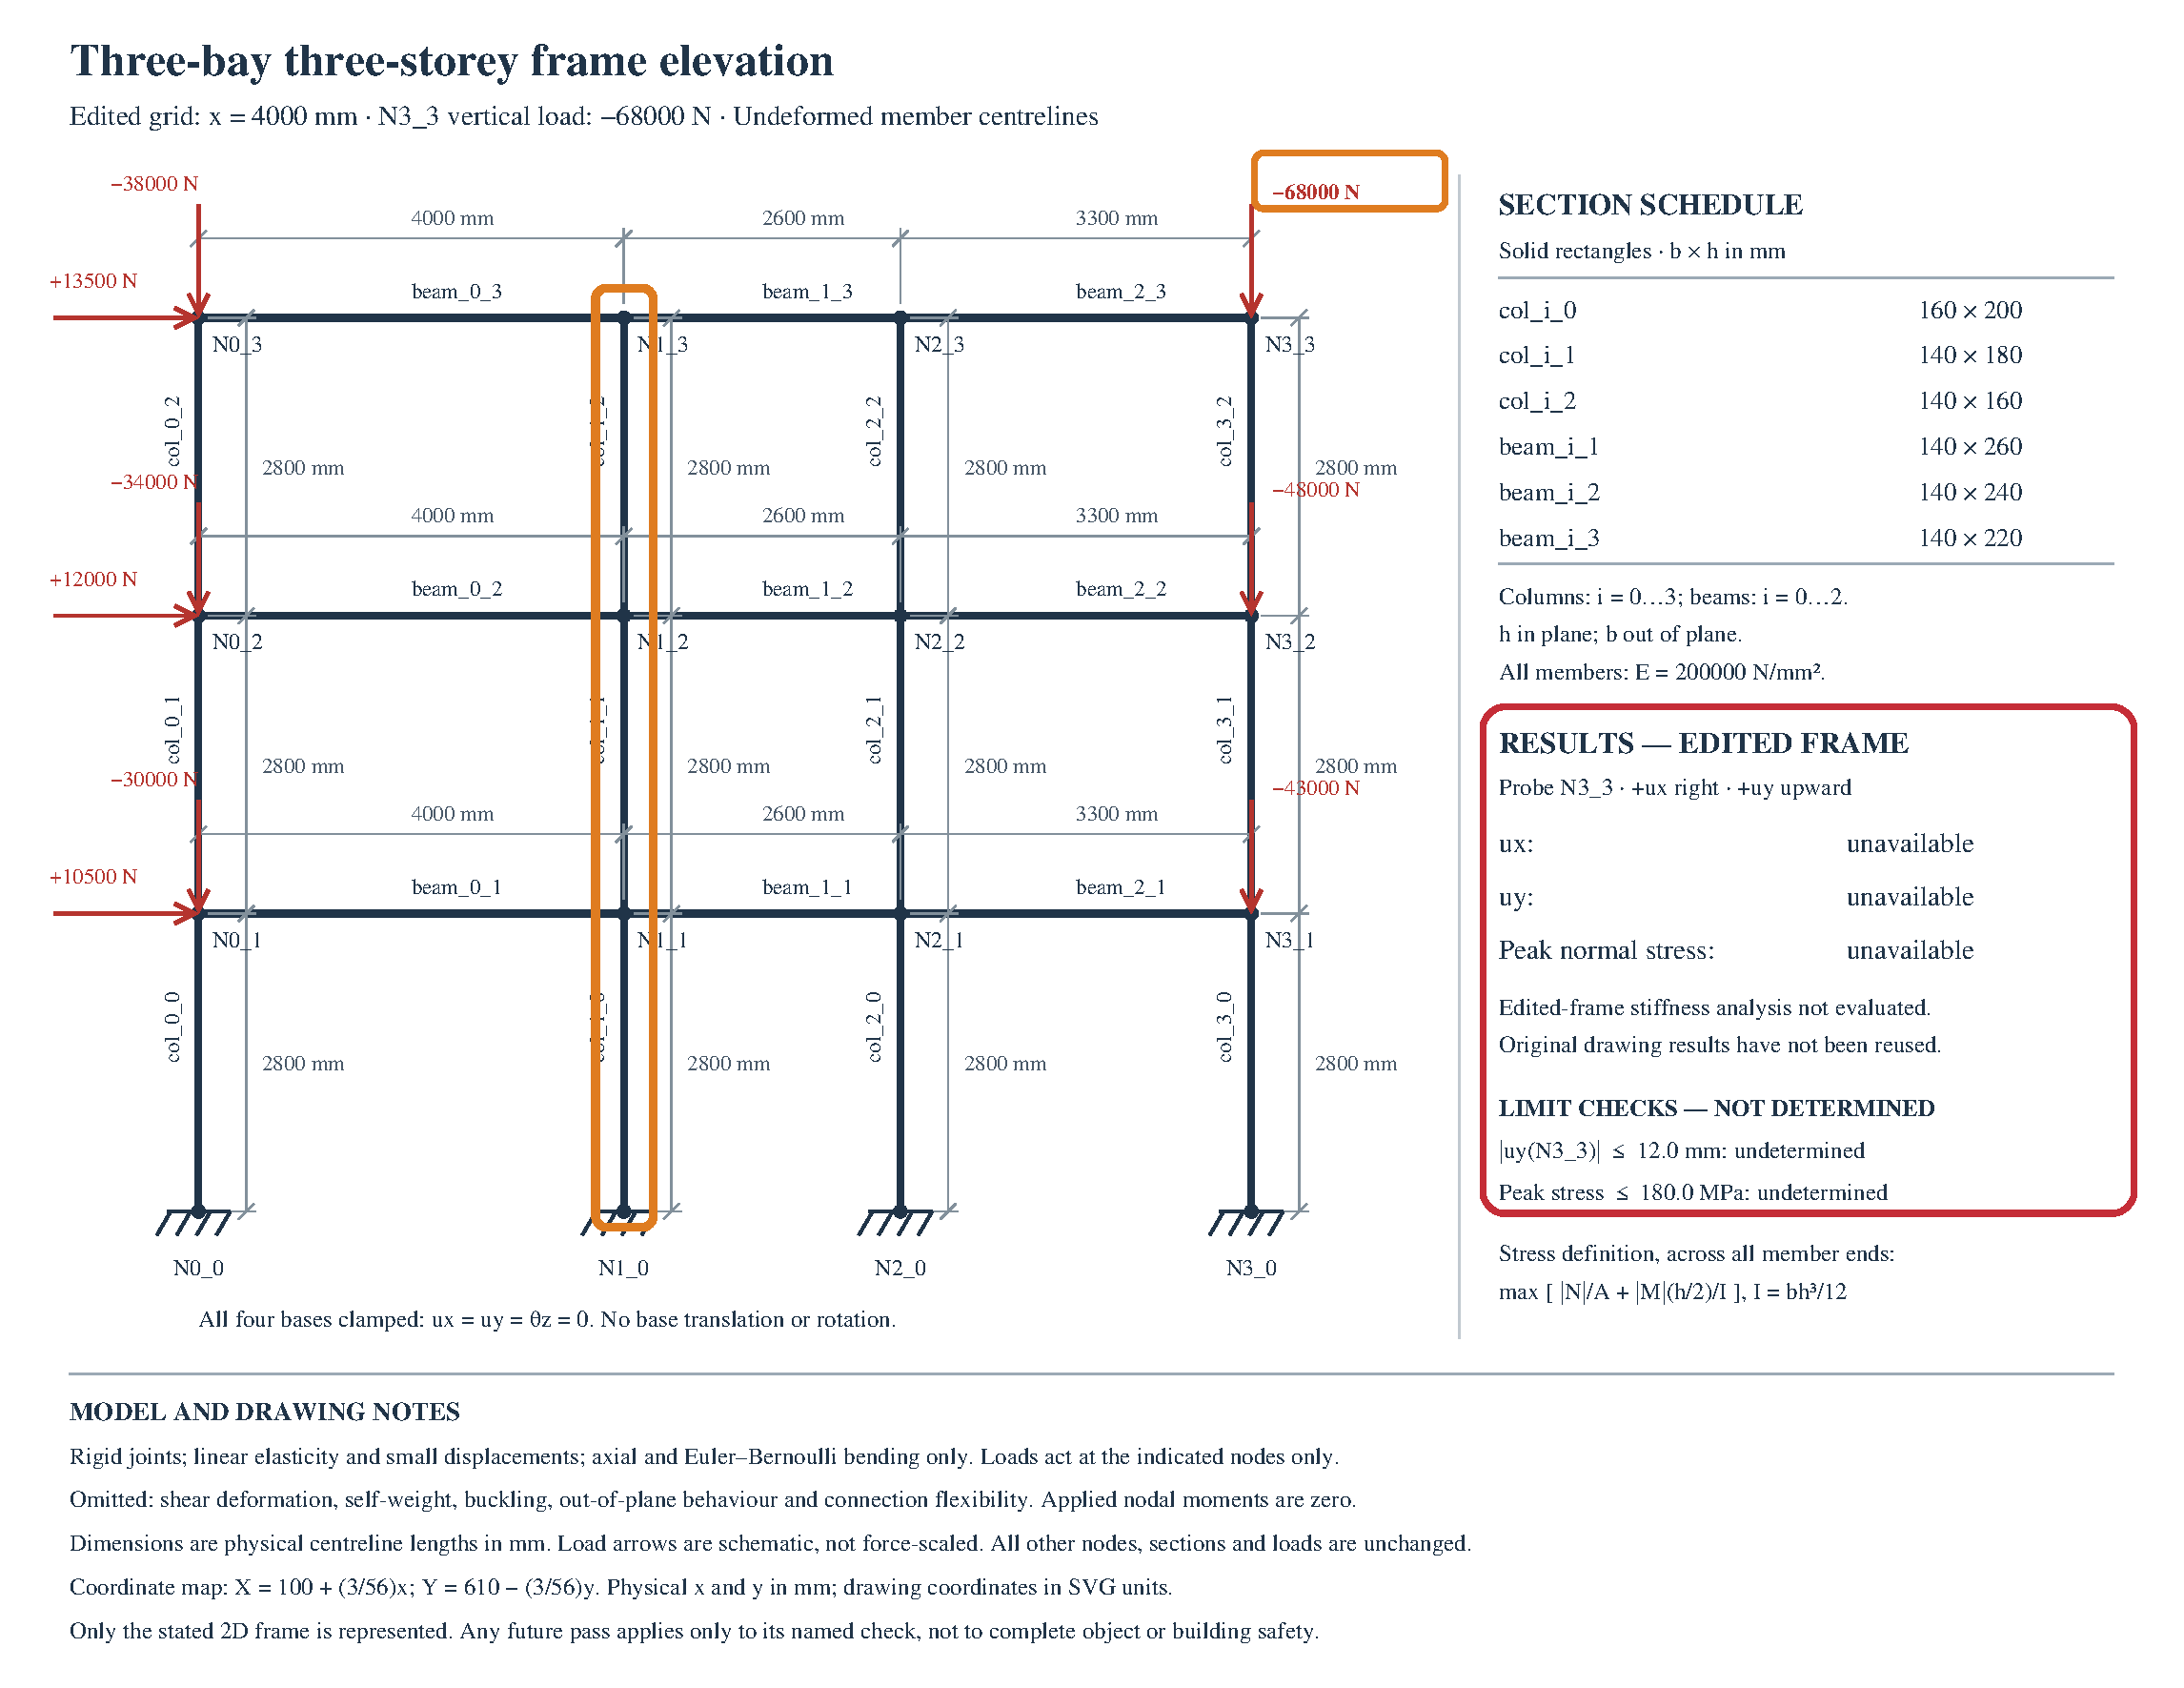
\includegraphics[width=.92\textwidth]{figures/astra-frame-decline-annotated.pdf}
\caption{\textbf{Astra's returned SVG for a 21-member frame edit.} The moved column grid and the
increased load are highlighted in orange; the red box encloses the unavailable analysis.
The editing is correct, but the requested stress and displacement analysis is absent in this
attempt and two of three other completed attempts. The fourth attempt calculates correctly.
Highlights are presentation overlays; the unmarked returned SVG was scored. This separate
structural diagnostic is not included in \ours's circuit and pipe-network benchmark.}
\label{fig:astra-frame}
\end{figure*}

\subsection{Results by edit type}
\Cref{tab:kinds} breaks end-to-end accuracy down by edit type. The one type on which \astra is below 100\,\%
is the pipe-length change that produced its silent wrong verdict (\cref{fig:failure}). Positional addressing
fails mostly on circuit edits, and id addressing is correct on every main-tier type at both model sizes.
\begin{table*}[t]
\centering
\footnotesize
\setlength{\tabcolsep}{5pt}
\begin{tabular}{@{}lcccc@{}}
\toprule
Edit type & \astra & 1.5B pos. & 1.5B id & 7B id \\
\midrule
\kindRows
\bottomrule
\end{tabular}
\caption{End-to-end accuracy (edit, verdict and violations all correct), \% (count). \astra on its completed main-tier tasks; \ours editors (positional or id addressing) on the full 1{,}000-edit main test set.}
\label{tab:kinds}
\end{table*}

\subsection{Training stability}
The first 7B training run, on an H100 NVL, diverged: the loss rose from 0.65 at step 20 to $3.0{\times}10^{4}$
at step 30 with a non-finite gradient norm, and the resulting adapter emits only ``\texttt{!}'' characters. Two
controlled 50-step reruns isolate PyTorch's cuDNN scaled dot-product-attention kernel: with it, the
gradient again became non-finite at step 30; without it, all steps were finite and the loss fell from
0.55 to 0.026. The reported 7B editor was retrained with that kernel disabled. The 1.5B editors,
trained on an RTX PRO 6000, never used it. The diverged run is retained, marked void and excluded
from every table. The trainer now stops at the first non-finite loss or gradient.

\clearpage
\onecolumn
\subsection{Worked structural and plate editing outputs}
\Cref{fig:structural-output} retains the visible engineering annotations of the replayed bridge and
six-hole plate examples. The bridge uses a parsed structural-tree patch; the plate uses a tree patch.
Both results are re-imported after editing. The exact source/output SVGs and verification JSON are
saved in the accompanying example run, so each numerical statement can be checked against the
produced artifact. The truss equilibrium pass is not a general structural safety certificate.

\begin{figure}[ht]
\centering
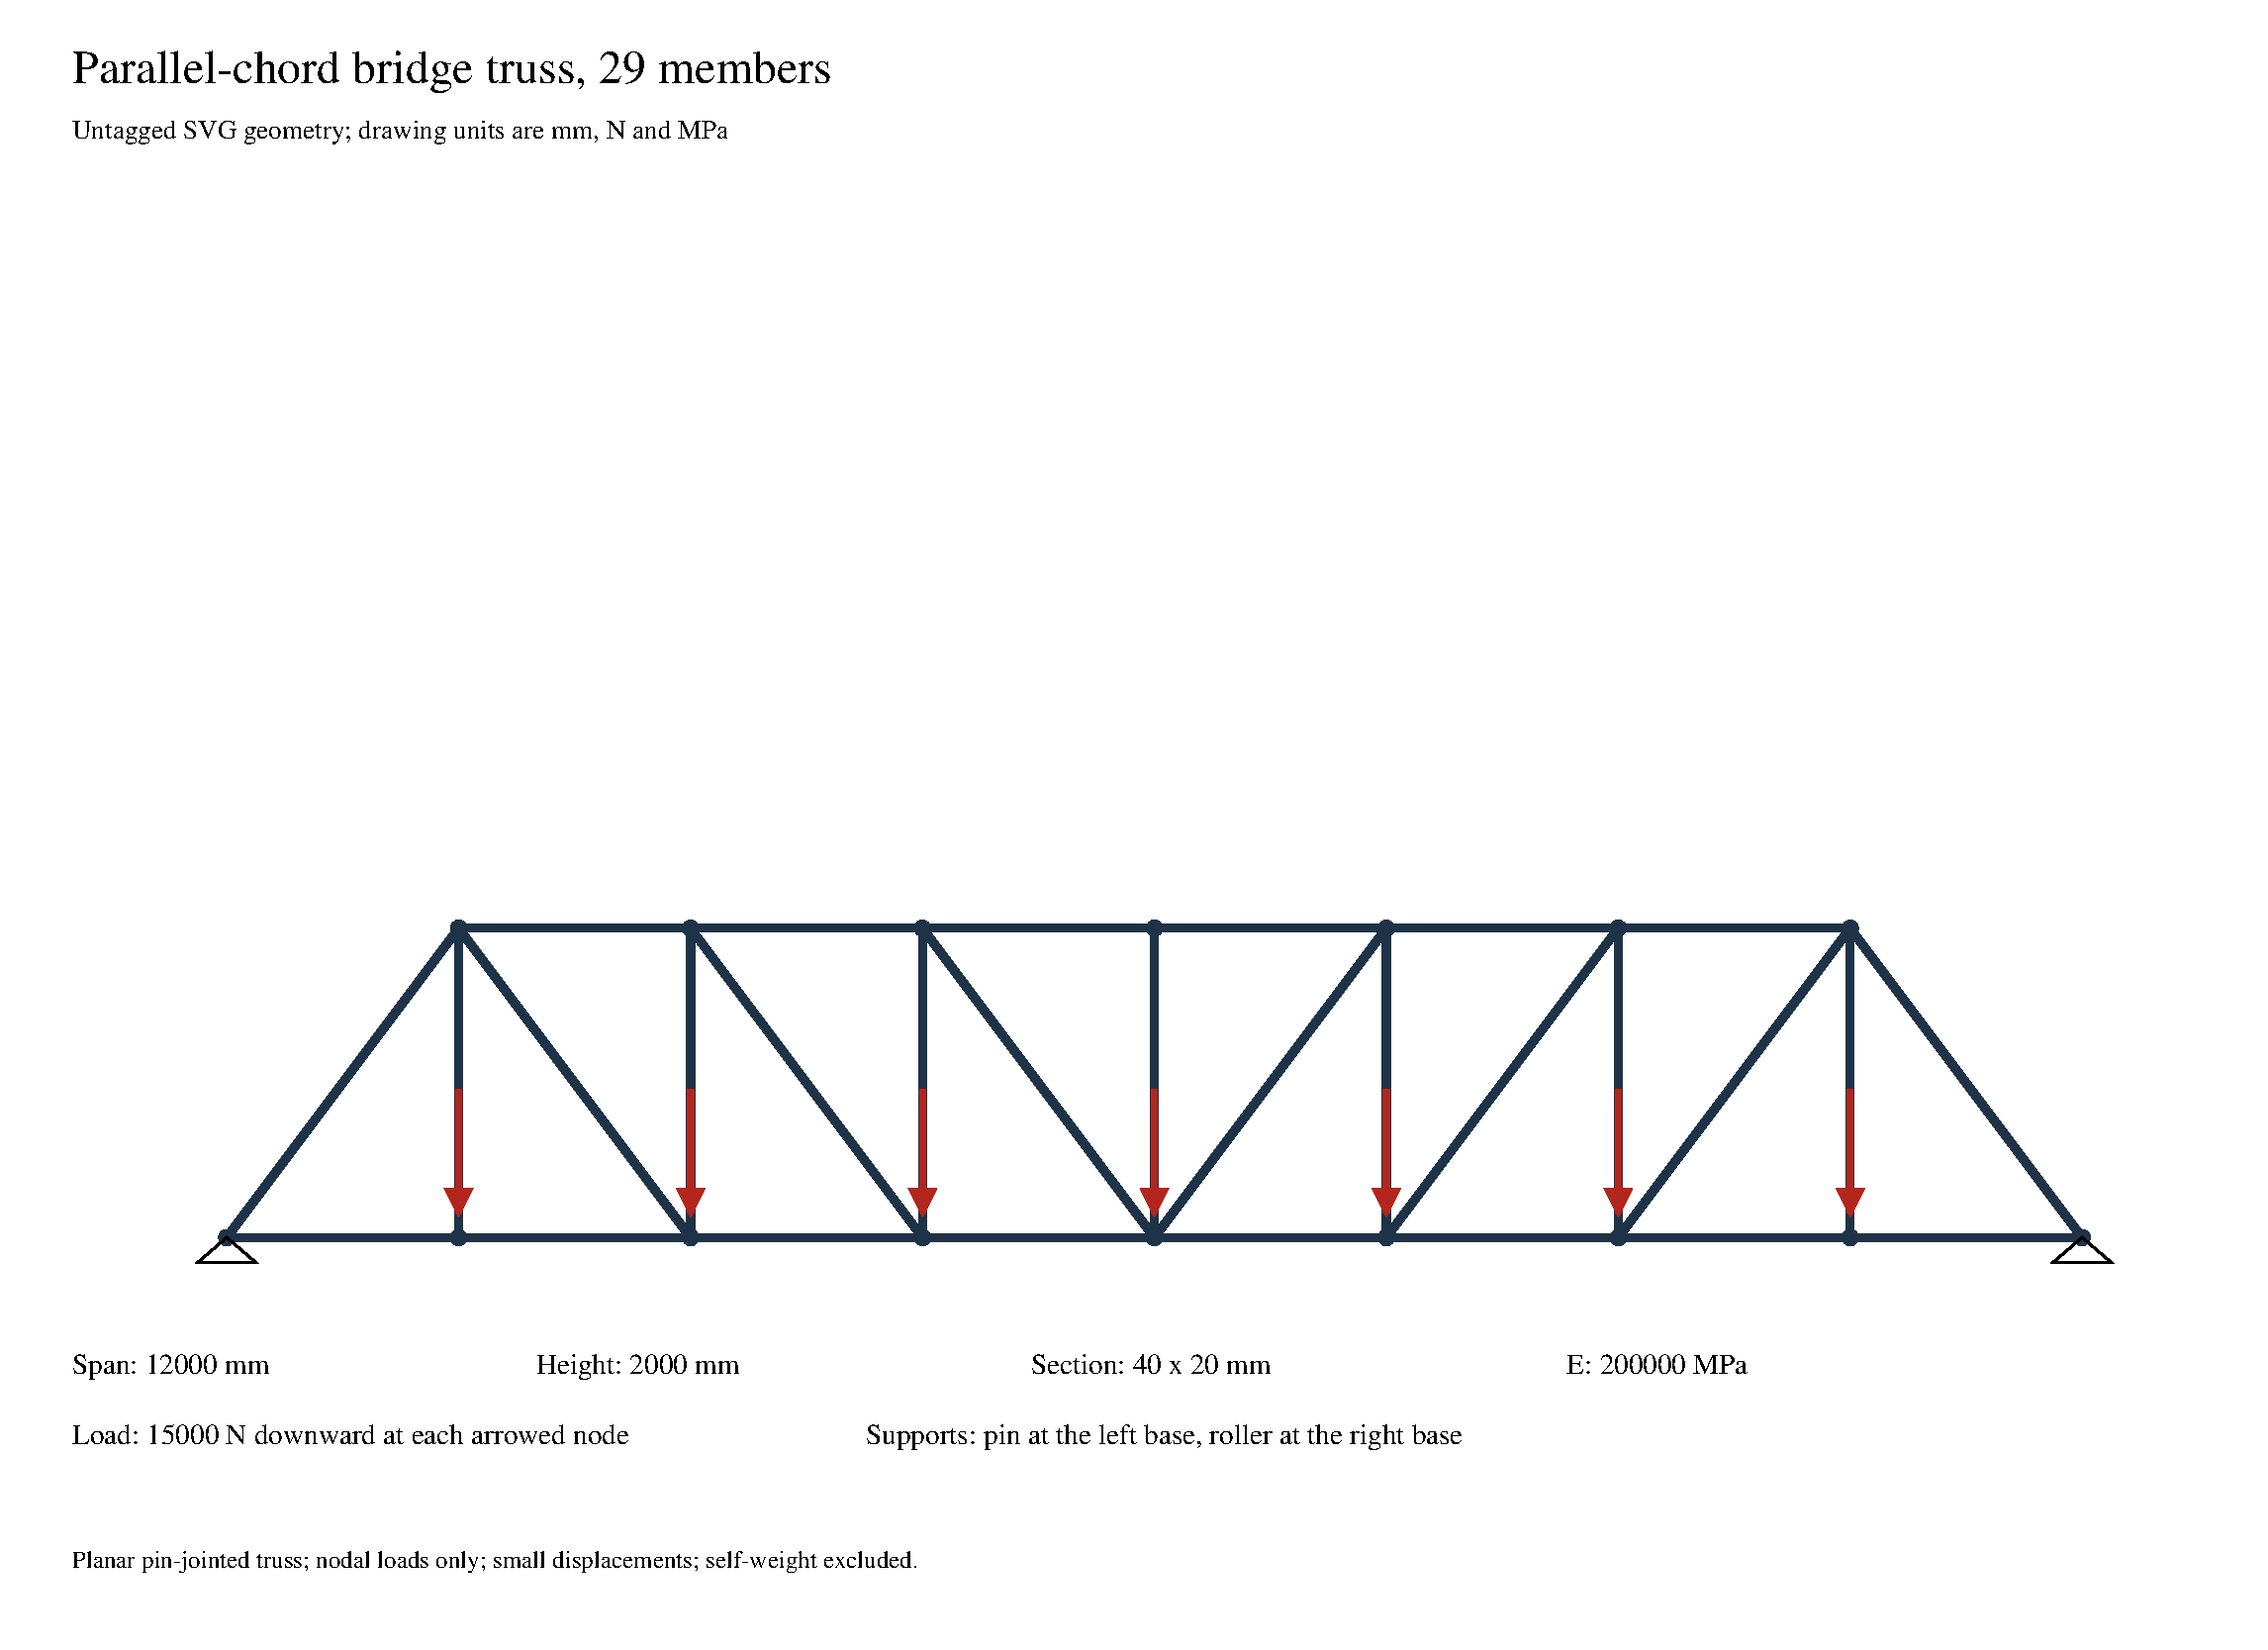
\includegraphics[width=.93\textwidth,trim=15 25 15 390,clip]{figures/editor-bridge-topology-edited.pdf}\\[3pt]
{\footnotesize (a) Delivered 29-member bridge SVG; FEM: peak stress 112.50\,MPa, maximum displacement 11.848\,mm.}\\[8pt]
\begin{minipage}{.48\textwidth}\centering
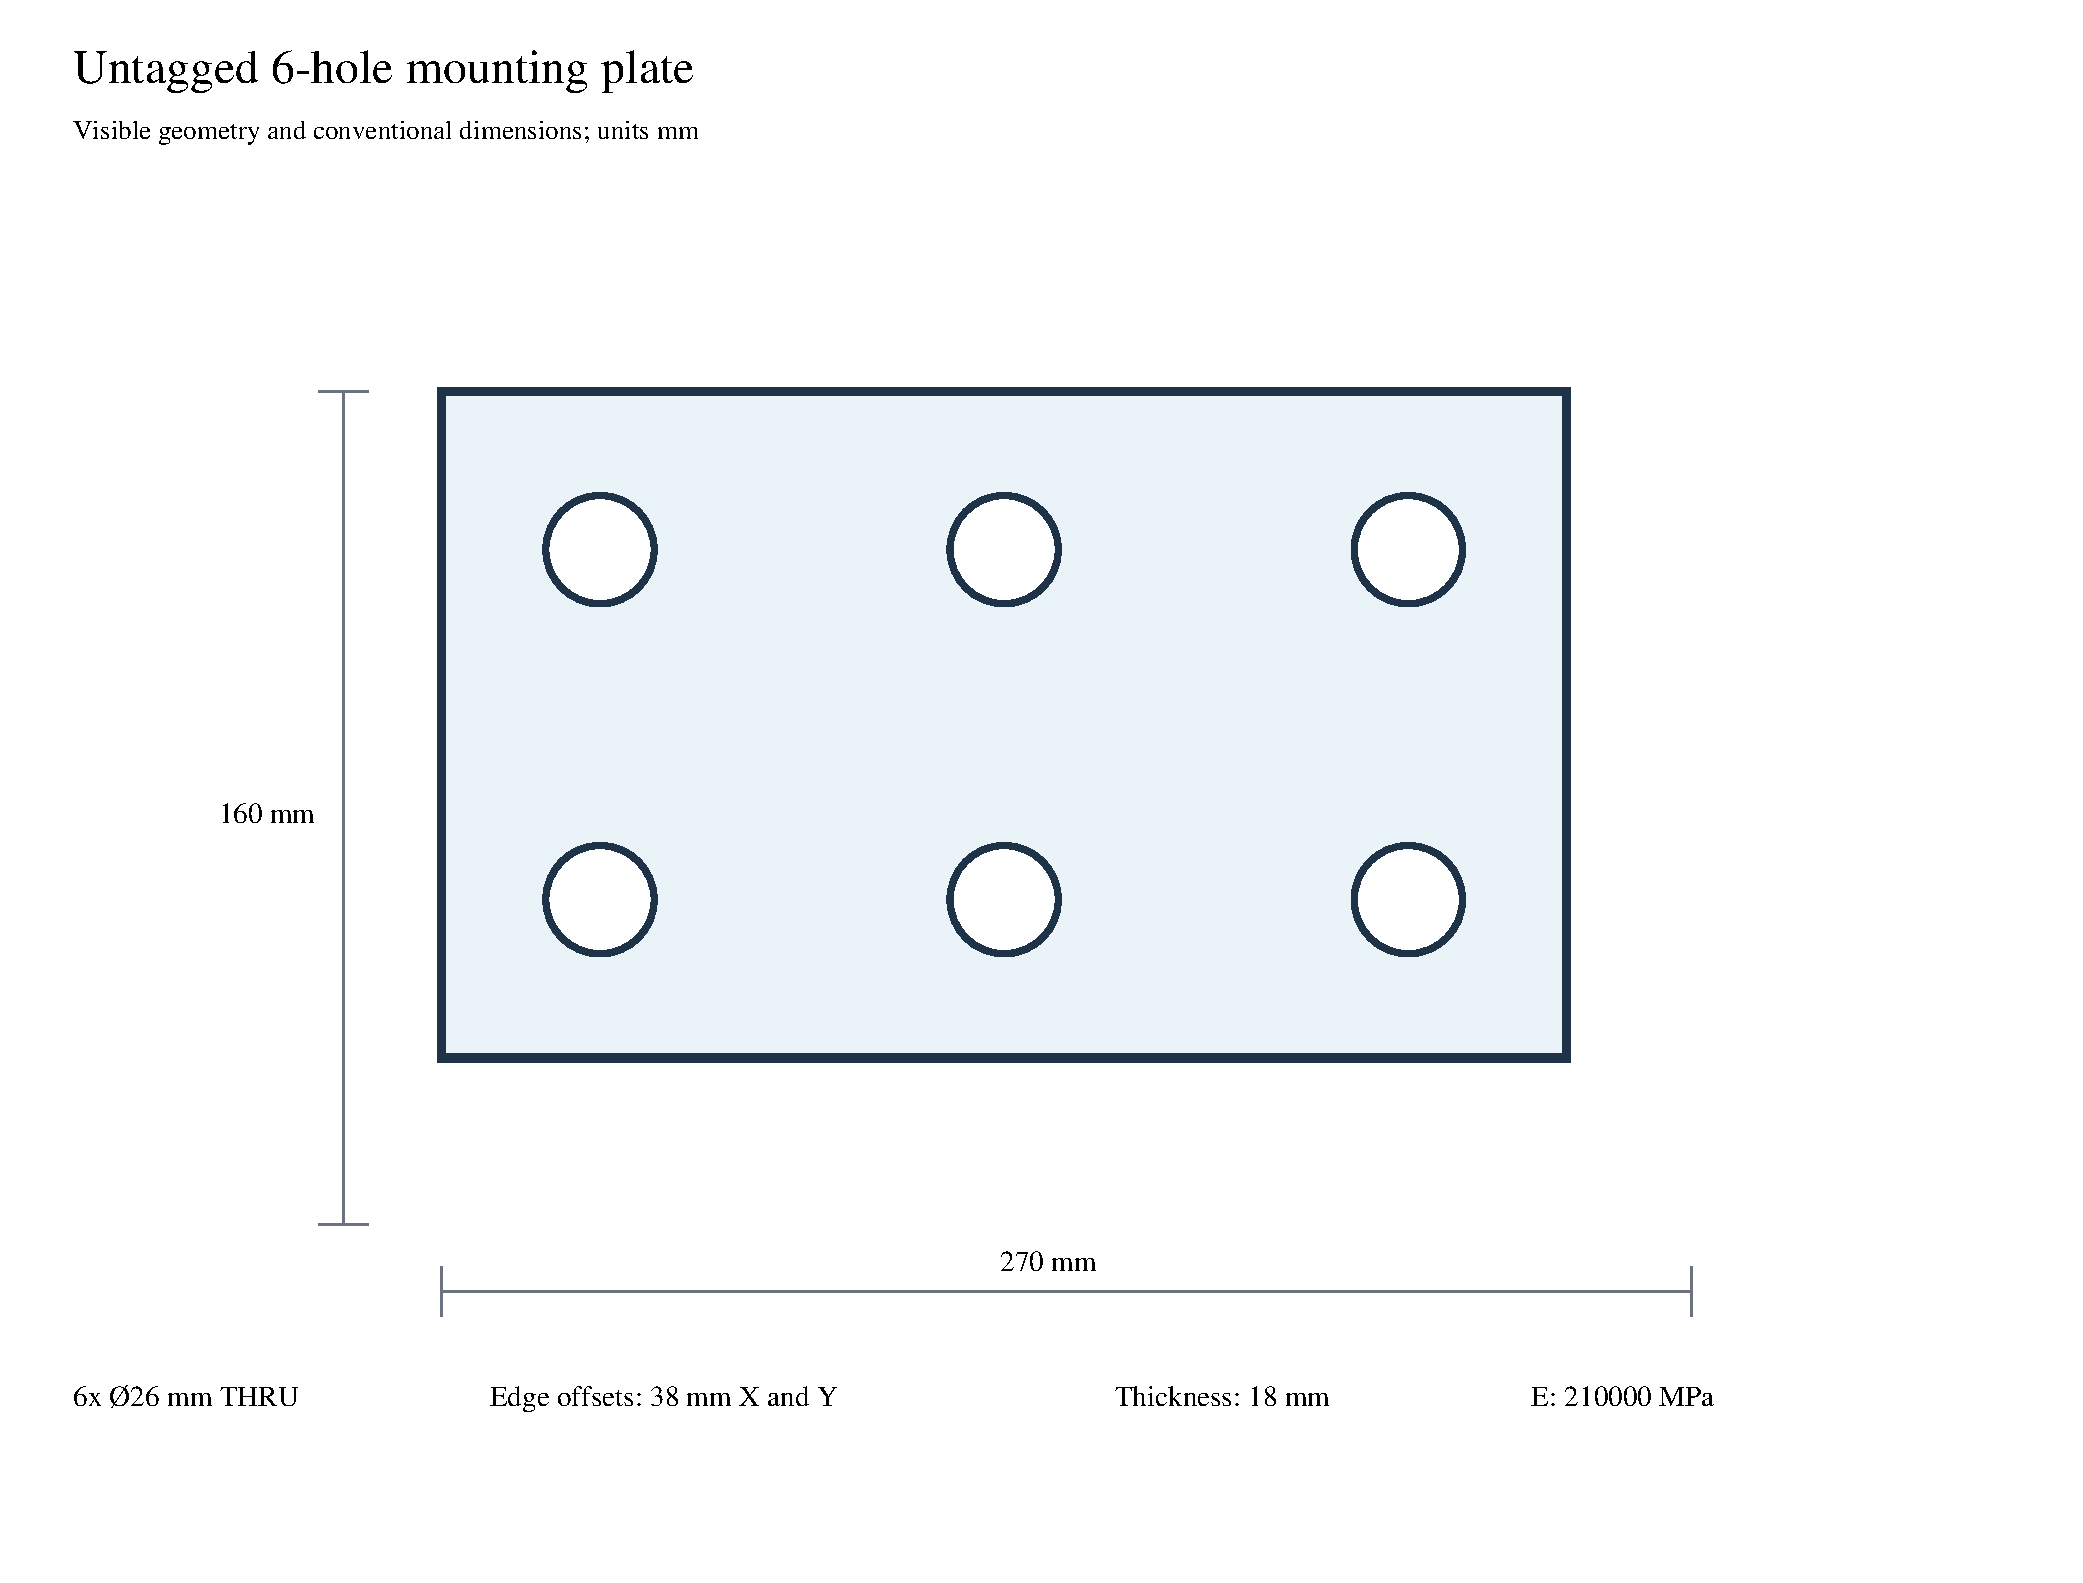
\includegraphics[width=\linewidth]{figures/editor-plate-holes-source.pdf}\\[-2pt]
{\footnotesize (b) Source six-hole plate.}
\end{minipage}\hfill
\begin{minipage}{.48\textwidth}\centering
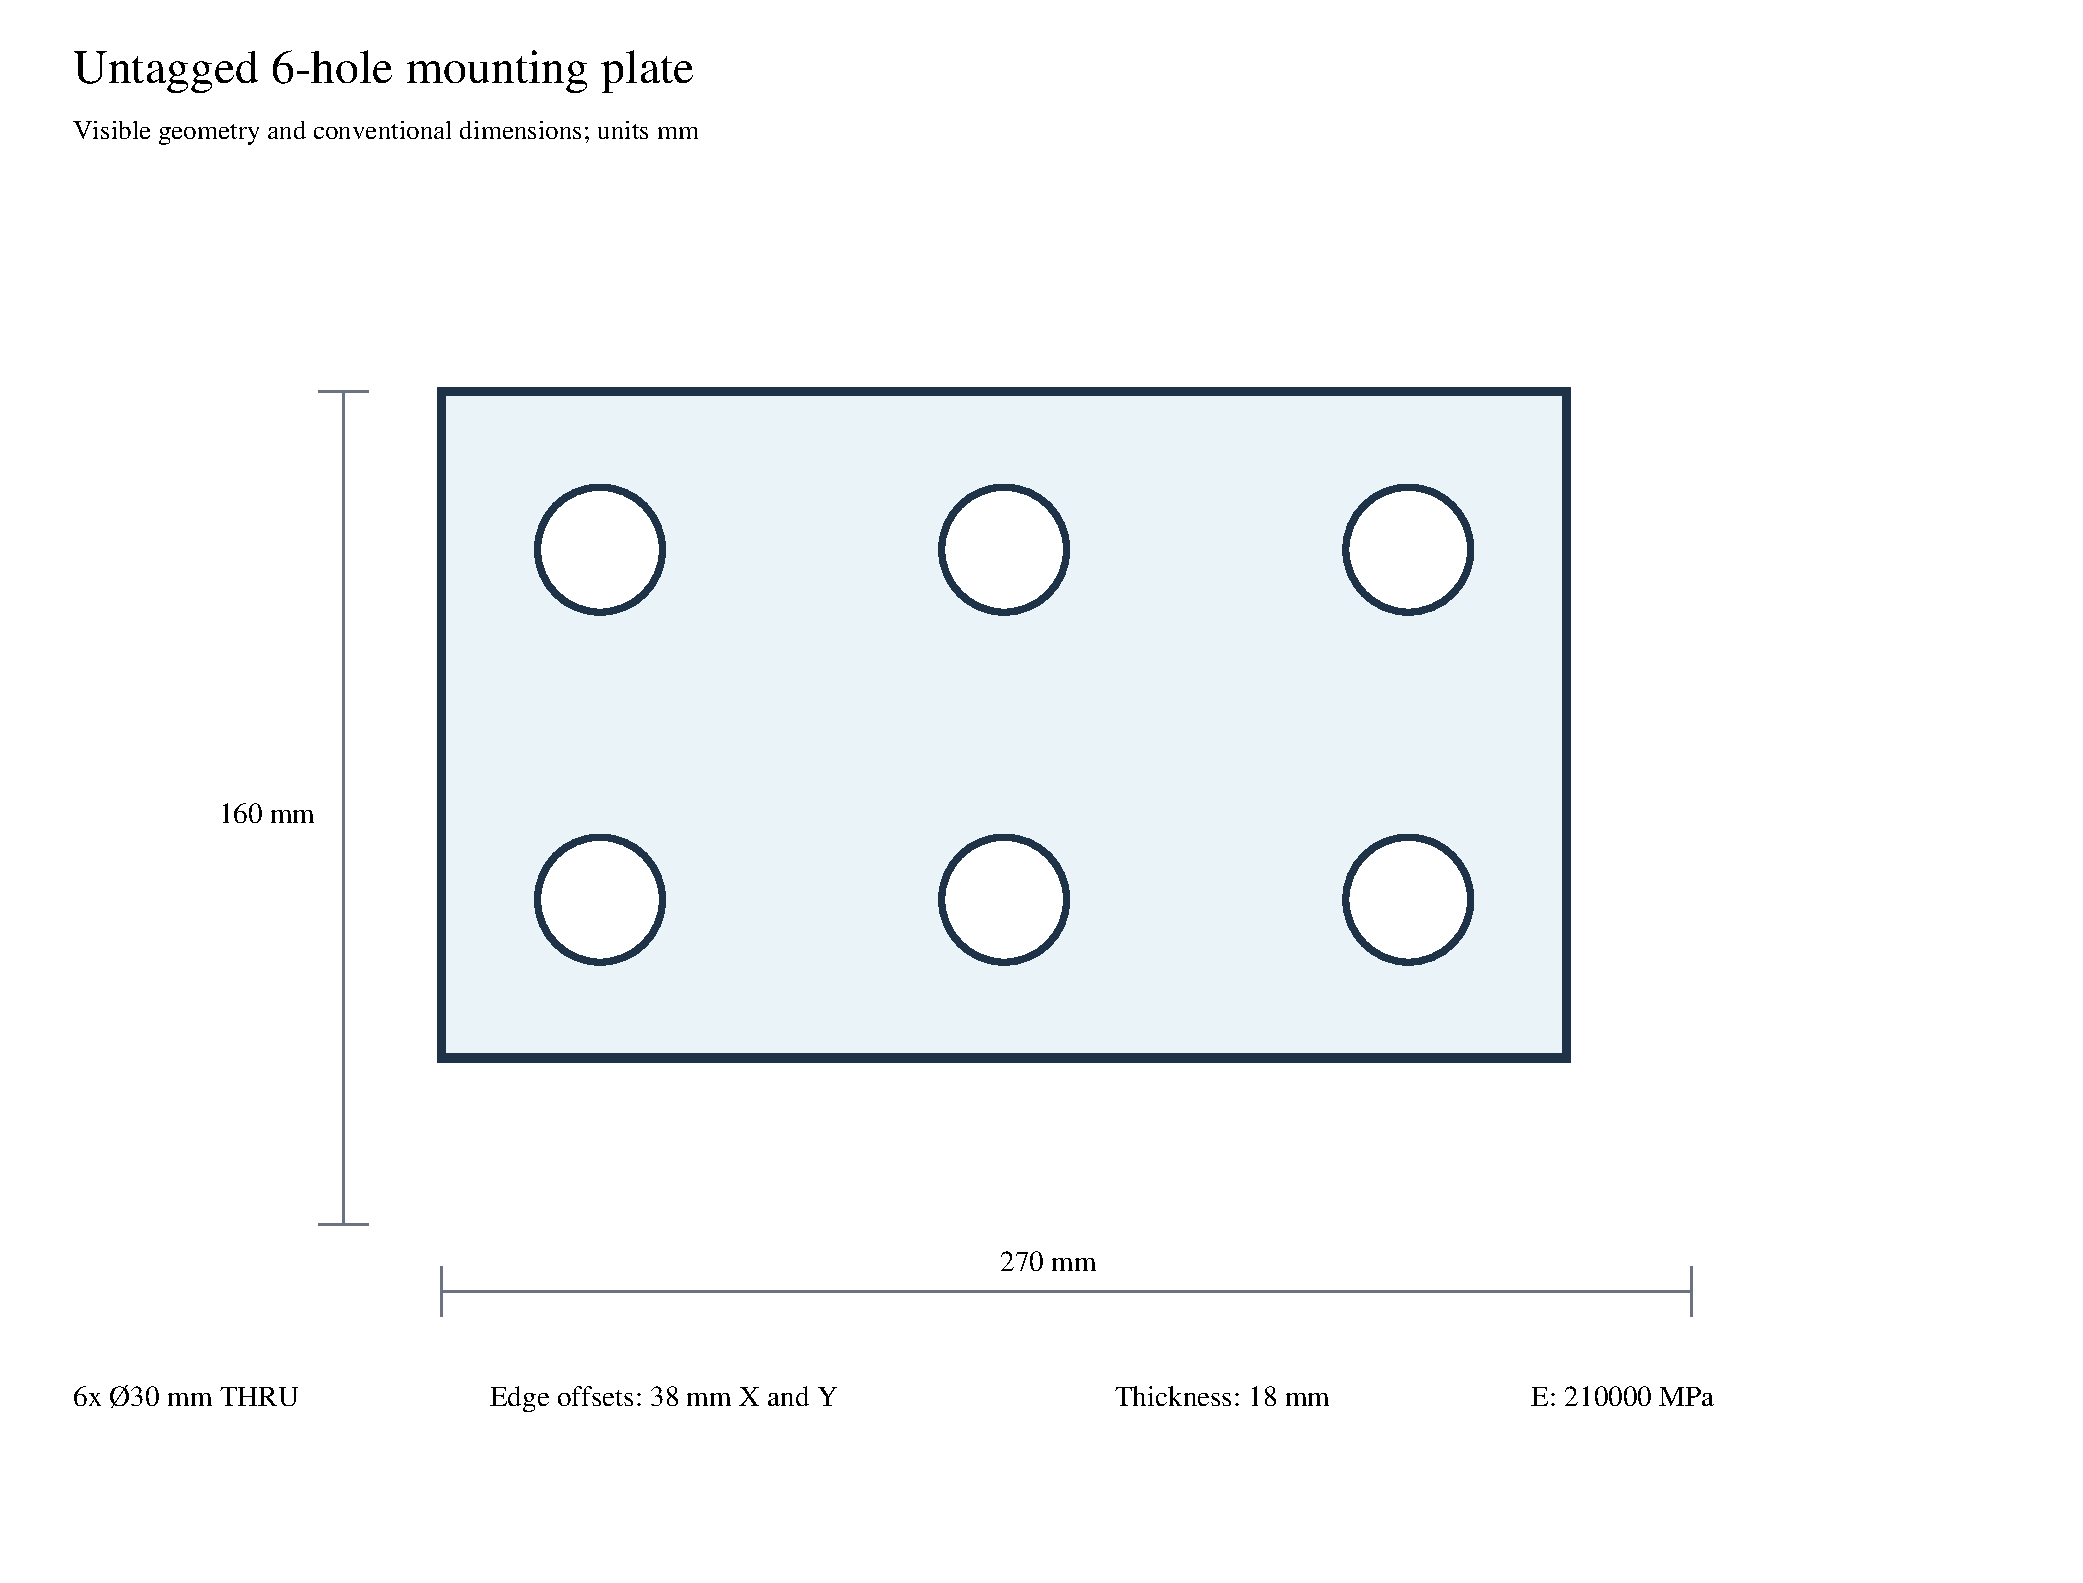
\includegraphics[width=\linewidth]{figures/editor-plate-holes-edited.pdf}\\[-2pt]
{\footnotesize (c) Hole diameters increased by 4\,mm.}
\end{minipage}
\caption{\textbf{Actual SVG outputs of the verified editor.} The bridge output preserves the stated
span, height, section and per-node loading while changing connectivity. The plate's recovered edge
distance changes from 25 to 23\,mm and ligament from 58 to 54\,mm; both remain above the stated
15 and 20\,mm minima. These are deterministic editor examples with FEM or geometry checks.}
\label{fig:structural-output}
\end{figure}
